\begin{answer}
	\begin{figure}[H]
		\centering
		\vspace{2mm}
		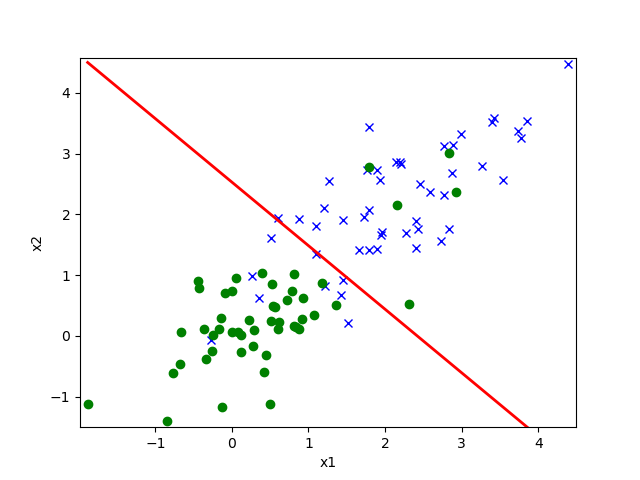
\includegraphics[width=0.65\linewidth]{../src/linearclass/logreg_pred_2.png}
		\centering
		\vspace{2mm}
		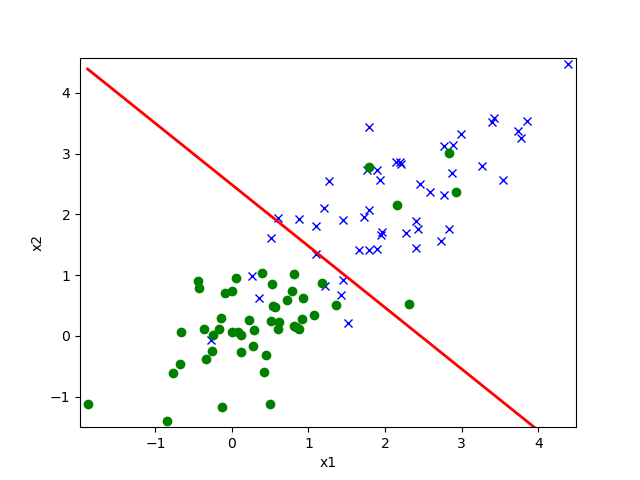
\includegraphics[width=0.65\linewidth]{../src/linearclass/gda_pred_2.png}
		\caption{Separating hyperplanes for logistic regression (top)
		and GDA (bottom) on Dataset 2.}
	\end{figure}

	GDA seems to perform worse than logistic regression on Dataset 1
	(GDA Accuracy: 0.81 and LR Accuracy: 0.83).
	This is probably because the $x^{(i)}$'s are not Gaussian. We
	saw in the notes that logistic regression is more robust than GDA
	when the underlying dataset is not drawn from a multivariate Gaussian.
\end{answer}
